\pagestyle{sebastian}
\section{Zustandsregler} \label{sec:Zustandsregler}
Der nachfolgende Zustandsregler basiert auf einer \textbf{einfachen Zustandsrückführung}, d.h. Änderungen innerhalb des Systems werden auf die vorher definierte Ruhelage ausgeregelt.

\subsection{Reglerentwurf}
\label{sec:Reglerentwurf}

\subsubsection{Nachweis der Steuerbarkeit}
\label{sec:Nachweis der Steuerbarkeit}

Zur Implementierung einer Reglerstruktur wird vorausgesetzt, dass das System steuerbar ist. Die vollständige Steuerbarkeit ist gegeben, wenn unter Berücksichtigung der Eingangsgröße $\underline{u}(t)$ das System von jedem beliebigen Anfangszustand $\underline{x}_{\mathrm{0}}$ in jeden beliebigen Endzustand $\underline{x}_{\mathrm{e}}$ überführt werden kann. Der Nachweis erfolgt über die Auswertung der \textbf{Steuerbarkeitsmatrix} $Q_{\mathrm{s}}$. Zur Berechnung werden die Systemmatrix $A$ und die Eingangsmatrix $B$ benötigt (\autoref{eq:Gleichung7.1}).

\begin{empheq}[box=\widefbox]{align}
    \underline{Q}_{\mathrm{s}} &= \left(\underline{B}\quad\underline{A}\cdot\underline{B}\quad ... \quad\underline{A}^{(n-1)}\cdot\underline{B}\right)
    \label{eq:Gleichung7.1}
\end{empheq}
\newline
Bei \textbf{SISO}- oder \textbf{SIMO}-Systemen folgt eine quadratische Matrix, d.h. die \textbf{Bedingung} für die Steuerbarkeit lautet:

\begin{align*}
    det(\underline{Q}_{\mathrm{s}}) \neq 0.
\end{align*}
\newline
Sofern ein \textbf{MISO}- oder \textbf{MIMO}-System vorliegt, muss der \textbf{Rang} gleich $n$ bzw. $m$ sein. Die Variablen $n$ und $m$ geben die Anzahl der linear unabhängigen Zeilen und Spalten wieder. \\
Falls

\begin{align*}
    n &> m: \\
    rank(\underline{Q}_{\mathrm{s}}) &= m
\end{align*}
\newline
oder
\begin{align*}
    n &< m: \\
    rank(\underline{Q}_{\mathrm{s}}) &= n
\end{align*}
\newline
gilt, ist das System steuerbar.

\clearpage

Durch \textbf{Anwendung} der Vorschrift aus \autoref{eq:Gleichung7.1} folgt die Steuerbarkeitsmatrix des inversen Pendels in der instabilen Ruhelage zu:

\begin{align*}
    \underline{Q}_{\mathrm{s}} &= 
    \begin{bmatrix}
        0 & -1.9548 & 24.5620 & -381.4330 \\
        -1.9548 & 24.5620 & -381.4330 & 4.5979\cdot 10^{3} \\
        0 & 113.0101 & -1.2831\cdot 10^{3} & 1.4670\cdot 10^{4} \\
        113.0101 & -1.2831\cdot 10^{3} & 1.4670\cdot 10^{4} & -1.6797\cdot 10^{5}
    \end{bmatrix}.
\end{align*}
\newline
Die Matrix ist quadratisch. Die \textbf{Determinante} folgt zu:

\begin{empheq}[box=\widefbox]{align}
    det(\underline{Q}_{\mathrm{s}}) \approx 12.24\cdot 10^{7}.
    \label{eq:Gleichung7.2}
\end{empheq}
\newline
Das implementierte System ist \textbf{steuerbar}.

\subsubsection{Reglergesetz}
\label{sec:Reglergesetz}

Das allgemeine \textbf{Reglergesetz} für die Zustandsrückführung ist nachfolgend gezeigt. Die Systemstruktur kann der \autoref{fig:Bild7.1} entnommen werden. Gleichungen zur Berechnung der Matrix $K$ folgen in \autoref{sec:LMI}.

\begin{empheq}[box=\widefbox]{align}
    \underline{u}(t) &= -\underline{K}\cdot\underline{x}(t)
    \label{eq:Gleichung7.3}
\end{empheq}

\begin{figure}[H]
    \centering
    \begin{tikzpicture}[framed][domain=0:0]
        % Umgebung
        \draw[thin,color=black] (-1,0);
        % Rechteck - Strecke
        \node at (3,0) [rectangle, draw, very thick] (strecke) {\Large Strecke};
        % Pfeil \underline{y}
        \draw[-{Implies}, double, very thick] (4.03,0) -- (4.7,0);
        % \underline{y}
        \node[text width=1cm] at (4.7, 0.3) {$\underline{y}$};
        % Rechteck - \underline{K}
        \node at (1.8,-3) [rectangle, draw, very thick] (k) {\Large $-\underline{K}$};
        % Pfeil \underline{x}
        \draw[double, very thick] (3.5,-0.37) -- (3.5,-2.99);
        \draw[-{Implies}, double, very thick] (3.46,-3) -- (2.45,-3);
        % Fix der Biegung des Pfeils für \underline{x}
        \draw[very thick] (3.46,-3.032) -- (3.55,-3.032);
        \draw[very thick] (3.532,-3.03) -- (3.532,-2.98);
        % \underline{x}
        \node[text width=1cm] at (4.2, -1.6) {$\underline{x}$};
        % Pfeil \underline{u}
        \draw[double, very thick] (1.13,-3) -- (0.265,-3);
        \draw[double, very thick] (0.25,-2.95) -- (0.2,-0.013);
        \draw[-{Implies}, double, very thick] (0.25,0) -- (1.98,0);
        % Fix der Biegung des Pfeils für \underline{x}
        \draw[very thick] (0.265,-3.032) -- (0.2,-3.032);
        \draw[very thick] (0.217,-3.032) -- (0.217,-2.95);
        \draw[very thick] (0.168,-0.02) -- (0.168,0.051);
        \draw[very thick] (0.168,0.032) -- (0.27,0.032);
        % \underline{x}
        \node[text width=1cm] at (0.27, -1.6) {$\underline{u}$};
        % Rechteck - Regler (grün)
        \draw [rectangle, draw, very thick, green, dashed] (0.7,-2.4) rectangle (3,-3.6);
        \node[text width=1cm, green] at (1.8, -4) {Regler};
    \end{tikzpicture}
    \caption[Systemstruktur mit einfacher Zustandsrückführung]{Systemstruktur mit einfacher Zustandsrückführung}
    \label{fig:Bild7.1}
\end{figure}

\subsubsection{Lineare Matrixungleichungen}
\label{sec:LMI}

Die Berechnung der Reglermatrix K wird mit \textbf{quadratischen Ljapunov-Funktionen} und der \textbf{exponentiellen Stabilität} motiviert. Im ersten Schritt werden die Polstellenregionen lediglich durch die Vorgabe einer Decay-Rate $\alpha$  eingeschränkt. Die \textbf{Linearen Matrixungleichungen (LMI)} sind in \autoref{eq:Gleichung7.4} dargestellt. Zur Visualisierung der Einschränkungen dient \autoref{fig:Bild7.2}. Das Lösen der LMI's, insbesondere der \autoref{eq:Gleichung7.5} erfolgt mithilfe der Matlab-Toolbox \textbf{Robust-Control-Toolbox} (Linear Matrix Inequalities).

\begin{align}
    \begin{split}
        \underline{0} &> \underline{A}\cdot\underline{X} + \underline{X}\cdot\underline{A}^T - \underline{B}\cdot\underline{M} -\underline{M}^T\cdot\underline{B}^T + 2\cdot\alpha\cdot\underline{X}\\\\
        \underline{X} &> \underline{0}
    \end{split}
    \label{eq:Gleichung7.4}
\end{align}
\newline
mit
\begin{empheq}[box=\widefbox]{align}
    \underline{K} &= \underline{M}\cdot\underline{X}^{-1}
    \label{eq:Gleichung7.5}
\end{empheq}

\begin{figure}[H]
    \centering
    \begin{tikzpicture}[framed][domain=0:0]
        % Umgebung
        \draw[very thin,color=black] (-0.1,-1.1);
        
        % Alpha-Grenze
        \draw[dashed] (-0.8,-4) -- (-0.8,4);            
        % Alpha-Pfeil
        \draw[-stealth] (0,-2.5) -- (-0.8,-2.5) node[midway, above] {$\alpha$};
        
        % Koordinatenursprung
        \node[text width=1cm] at (0.6, -0.3) {0};

        % X-Achse
        \draw[->] (-4.2,0) -- (2,0) node[right] {$Re$}; 
        % Y-Achse
        \draw[->] (0,-4) -- (0,4) node[above] {$Im$};
        
        \begin{scope}
            % Clipping Maske zur Begrenzung
            \clip (-5,-4) rectangle (-0.8,4);
            
            % Bereich füllen
            \draw[pattern={crosshatch}, pattern color=grey, draw = white] (-4.0, -4.5) rectangle (3.2, 9);
        \end{scope}

        % Beschriftung des Polstellenbereichs
        \node[text width=3cm] at (-1.2,0.5) {$S(\alpha)$};
    \end{tikzpicture}
    \caption[Einschränkung der Polregion bei exponentieller Stabilität]{Einschränkung der Polregion bei exponentieller Stabilität zu $S(\alpha)$}
    \label{fig:Bild7.2}
\end{figure}

Sofern die Einschränkung mittels Decay-Rate nicht ausreicht, um die Voraussetzungen aus \autoref{sec:Einfuehrung} zu erreichen, werden zusätzliche LMI's eingeführt, welche weitere Einschränkungen mittels Kegel und Halbkreis vornehmen (\autoref{eq:Gleichung7.6} und \autoref{fig:Bild7.3}).

\begin{align}
    \begin{split}
        \underline{0} &> \underline{A}\underline{X} + \underline{X}\underline{A}^T - \underline{B}\underline{M} -\underline{M}^T\underline{B}^T + 2\alpha\underline{X}\\\\
        \underline{0} &>
        \begin{pmatrix}
            (\underline{A}\underline{X} + \underline{X}\underline{A}^T - \underline{B}\underline{M} - \underline{M}^T\underline{B}^T)\sin\theta & (\underline{A}\underline{X} - \underline{X}\underline{A}^T - \underline{B}\underline{M} + \underline{M}^T\underline{B}^T)\cos\theta \\\\
            (\underline{X}\underline{A}^T - \underline{A}\underline{X} + \underline{B}\underline{M} - \underline{M}^T\underline{B}^T)\cos\theta & (\underline{A}\underline{X} + \underline{X}\underline{A}^T - \underline{B}\underline{M} - \underline{M}^T\underline{B}^T)\sin\theta
        \end{pmatrix}\\\\
        \underline{0} &> 
        \begin{pmatrix}
            -r\underline{X} & \underline{A}\underline{X} - \underline{B}\underline{M} \\\\
            \underline{X}\underline{A}^T - \underline{M}^T\underline{B}^T & -r\underline{X}
        \end{pmatrix} \\\\
        \underline{X} &> \underline{0}
    \end{split}
    \label{eq:Gleichung7.6}
\end{align}

\begin{figure}[H]
    \centering
    \begin{tikzpicture}[framed][domain=0:0]
        % Umgebung
        \draw[very thin,color=black] (-0.1,-1.1);       
        % Halbkreis
        \draw[dashed] (0,-3) arc(270:90:3) -- cycle;
        
        % r-Pfeil
        \draw[-stealth] (0,0) -- (-1.24,2.74);      
        
        % r
        \node[text width=1cm] at (0, 1.6) {$r$};    
        
        % Alpha-Grenze
        \draw[dashed] (-0.8,-4) -- (-0.8,4);        
        
        % +Theta-Grenze
        \draw[dashed] (0,0) -- (-3,3);              
        
        % -Theta-Grenze
        \draw[dashed] (0,0) -- (-3,-3);                 
        % Alpha-Pfeil
        \draw[-stealth] (0,-2.5) -- (-0.8,-2.5) node[midway, above] {$\alpha$};
        
        % Koordinatenursprung
        \node[text width=1cm] at (0.6, -0.3) {0};       
        % Theta-Pfeil
        \draw[-stealth] (-0.7,0) to [bend left] (-0.5,0.5);
        
        % Theta
        \node[text width=1cm] at (-0.1, 0.2) {$\theta$};
        
        \begin{scope}
            % Clipping Maske zur Begrenzung
            \clip (-5,-4) rectangle (-0.8,4);
            
            % Bereich füllen
            \draw[pattern={crosshatch}, pattern color=grey] (0,0) -- (-2.12,2.12) arc[start angle=135, delta angle=90,radius=3] -- (0,0);
        \end{scope}
        
        % rechte Begrenzung 
        \draw[] (-0.8,-0.8) -- (-0.8,0.8);             
        
        % Beschriftung des Polstellenbereichs
        \node[text width=3cm] at (-1.2,0.5) {$S(\alpha,r,\theta)$};
        
        % X-Achse
        \draw[->] (-4.2,0) -- (2,0) node[right] {$Re$}; 
        % Y-Achse
        \draw[->] (0,-4) -- (0,4) node[above] {$Im$};
    \end{tikzpicture}
    \caption[Einschränkung der Polregion bei Erweiterung der LMI]{Einschränkung der Polregion bei Erweiterung der LMI zu $S(\alpha,r,\theta)$}
    \label{fig:Bild7.3}
\end{figure}

\subsection{Reglervalidierung am linearen Modell}
\label{sec:Reglervalidierung}

Um eine geeignete Reglerstruktur zu entwerfen, werden zuerst die \textbf{Polstellen der Systemmatrix A} bestimmt und grafisch dargestellt (\autoref{fig:Bild7.4}). Aus der Abbildung geht hervor, dass zwei der vier rein reelen Polstellen instabil sind, da diese eine Realteil größer oder gleich Null aufweisen. Dies hat ein instabiles Systemverhalten zur Folge.

\begin{align*}
    eig(\underline{A}) &=
    \begin{bmatrix}
        0 \\
        6.5169 \\
        -7.5606 \\
        -11.5214
    \end{bmatrix}
\end{align*}

\begin{figure}[H]
   \centering
   \fbox{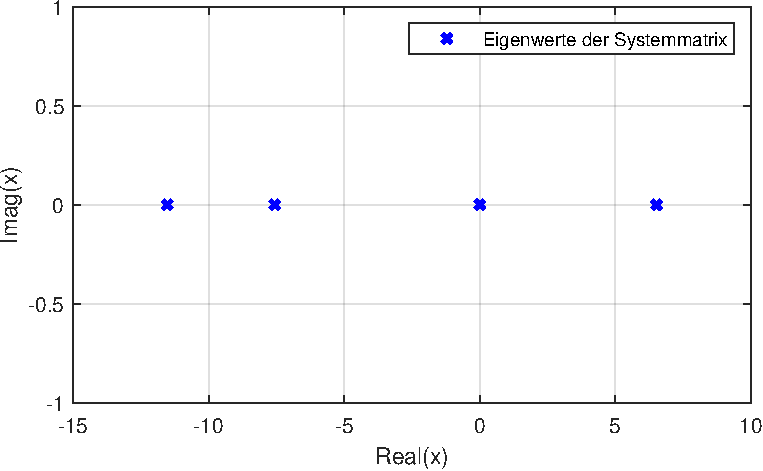
\includegraphics[width=0.8\textwidth]{Bilder/7_zustandsregler/Polstellen_der_Systemmatrix.pdf}}
   \caption[Polstellen der Systemmatrix]{Polstellen der Systemmatrix}
   \label{fig:Bild7.4}
\end{figure}

Der zu entwerfender Regler muss in der Lage sein, die maximal zulässige Eingangsspannung von $V_{\mathrm{m,Max}} = 20V$ auszureizen, jedoch nicht zu überschreiten, um größtmögliche Winkeländerungen von der definierten instabilen Ruhelage ausgleichen zu können. Die Simulationen werden mithilfe der Matlab-Erweiterung \textbf{Simulink} durchgeführt. Die Reglerstruktur ist in \autoref{fig:Bild7.5} dargestellt. Das linearisierte Zustandsraummodell verwendet gemäß Definition Delta-Größen, welche bei der Anwendung des linearen Reglers am nichtlinearen Modell berücksichtigt werden müssen. Da die entstehende K-Matrix eine Größe von (1x4) besitzt, wird fortan die Vektorschreibweise $k$ bevorzugt.

\begin{figure}[H]
   \centering
   \fbox{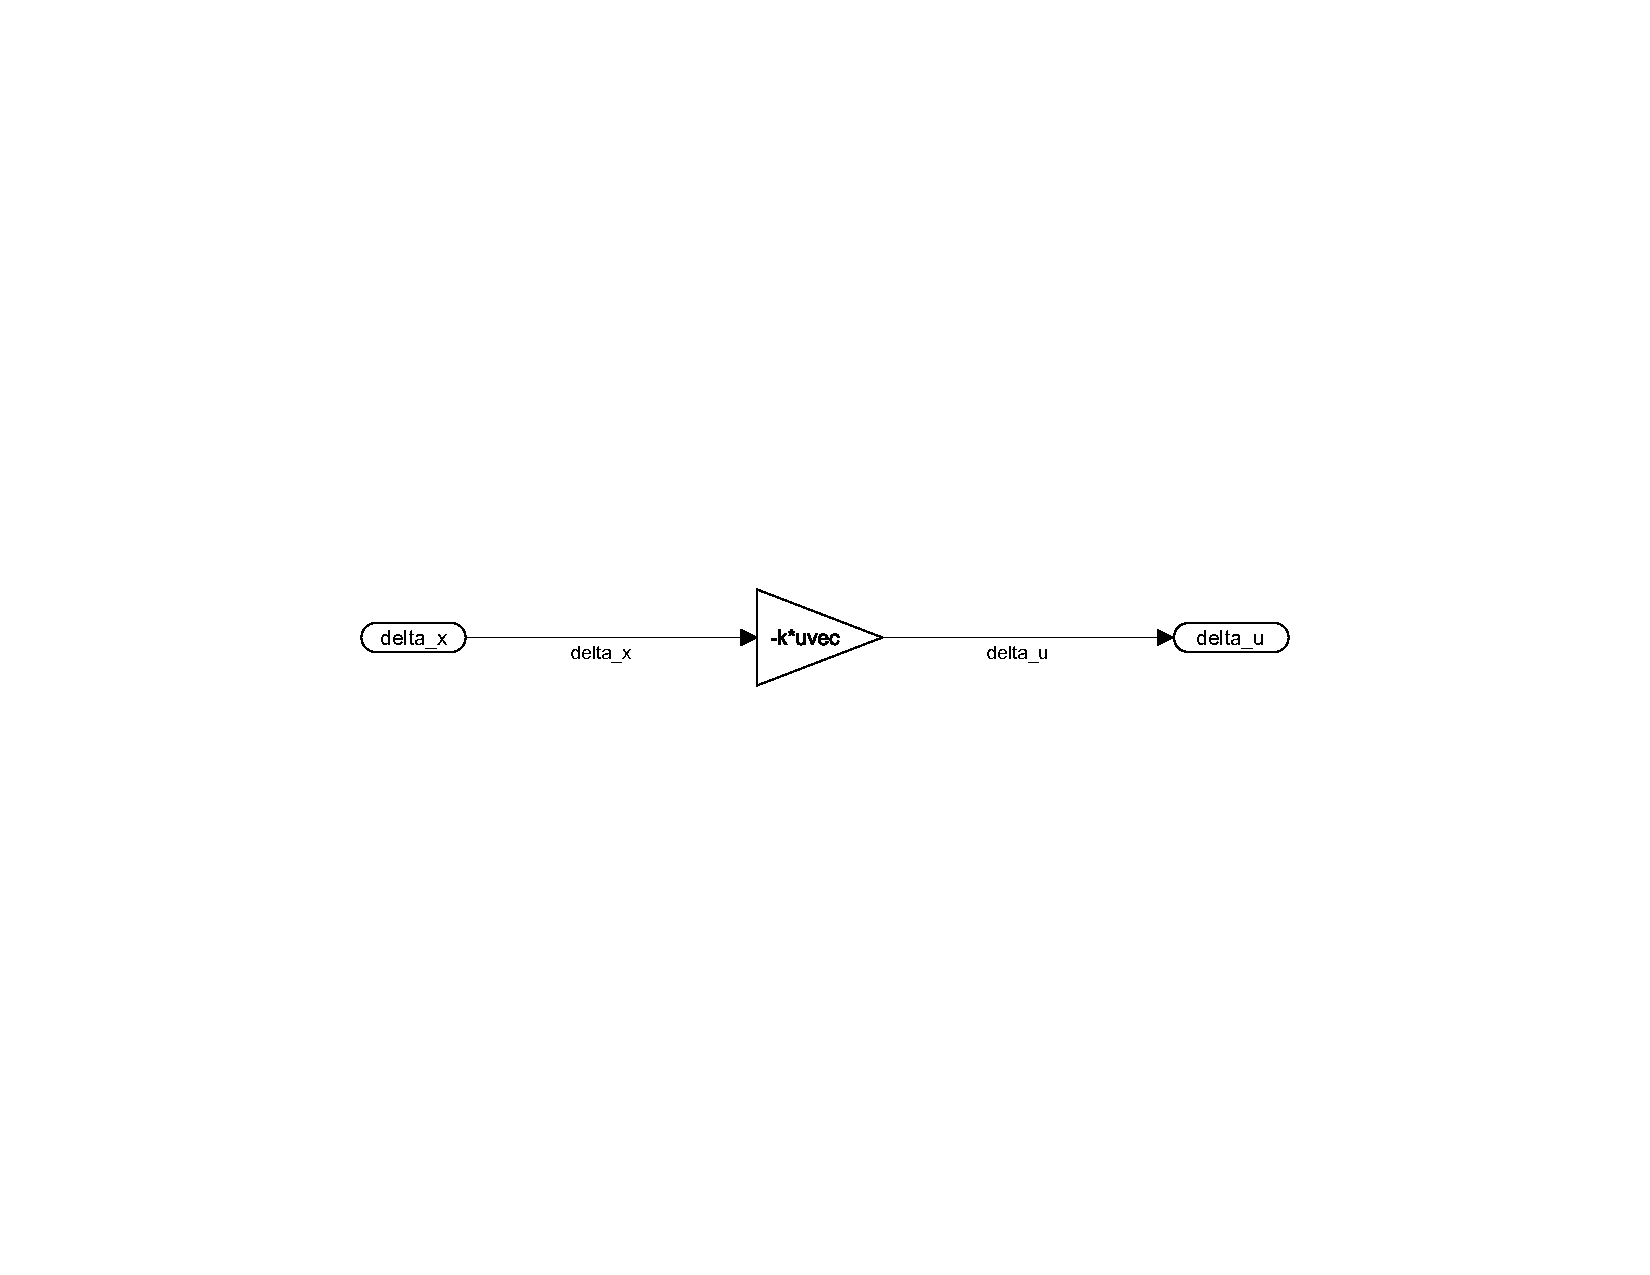
\includegraphics[width=0.95\textwidth]{Bilder/7_zustandsregler/Reglerstruktur_Simulink.pdf}}
   \caption[Simulink-Reglerstruktur]{Simulink-Reglerstruktur}
   \label{fig:Bild7.5}
\end{figure}

Im ersten Versuch wird nur die Decay-Rate $\alpha$ variiert (vgl. \autoref{fig:Bild7.2}). Der Startwinkel des Pendels wird von 15$^\circ$ solange verringert, bis der Maximalwert der anliegenden Eingangsspannung $V_{\mathrm{m}} \leq 20V$ erreicht. Zur Übersicht der Ergebnisse dient \autoref{tab:Tabelle7.1}.

\renewcommand{\arraystretch}{1.2}
\begin{table}[H]
    \centering
    \begin{tabular}{|c|c|c|c|c|c|c|}
        \hline
        & & \multicolumn{5}{c|}{ \boldmath{$\alpha$} } \\
        \makecell{\textbf{Anfangsauslenkung} \\ \textbf{Pendel [$^\circ$]}} & \textbf{Kriterium} & \textbf{1.0} & \textbf{0.5} & \textbf{0.3} & \textbf{0.1} & \textbf{0.05} \\
        \hline
        \multirow{2}{*}{15} & $V_{\mathrm{m,Max}}$ [V] & 39.107 & 31.983 & 29.184 & 26.471 & 27.351 \\
        & $V_{\mathrm{m,Max}} \leq$ 20V & - & - & - & - & -\\
        \hline
        \multirow{2}{*}{14} & $V_{\mathrm{m,Max}}$ [V] & 36.500 & 29.851 & 27.238 & 24.706 & 25.528 \\
        & $V_{\mathrm{m,Max}} \leq$ 20V & - & - & - & - & -\\
        \hline
        \multirow{2}{*}{13} & $V_{\mathrm{m,Max}}$ [V] & 33.893 & 27.719 & 25.293 & 22.941 & 23.704 \\
        & $V_{\mathrm{m,Max}} \leq$ 20V & - & - & - & - & -\\
        \hline
        \multirow{2}{*}{12} & $V_{\mathrm{m,Max}}$ [V] & 31.286 & 25.587 & 23.347 & 21.177 & 21.881 \\
        & $V_{\mathrm{m,Max}} \leq$ 20V & - & - & - & - & -\\
        \hline
        \multirow{2}{*}{11} & $V_{\mathrm{m,Max}}$ [V] & 28.679 & 23.454 & 21.401 & 19.412 & 20.057 \\
        & $V_{\mathrm{m,Max}} \leq$ 20V & - & - & - & X & -\\
        \hline
    \end{tabular}
    \caption[Auswertung von $V_{\mathrm{m}}$ für unterschiedliche Anfangsauslenkungen]{Auswertung der Eingangsspannung $V_{\mathrm{m}}$ für unterschiedliche Anfangsauslenkungen des Pendels bei Vorgabe einer Decay-Rate $\alpha$ [$\textbf{X}$ - erfüllt, $\textbf{-}$ - nicht erfüllt]} 
    \label{tab:Tabelle7.1}
\end{table}
\renewcommand{\arraystretch}{1}

Aus der Tabelle geht hervor, dass erst bei einem Anfangswinkel von 11$^\circ$ und $\alpha = 0.1$ die Spannung $V_{\mathrm{m}}$ unter 20V sinkt. Mithilfe der erweiterten LMI's wird nun versucht, ein größeren Startwinkel zu ermöglichen und weiterhin die Constraints einzuhalten. Dafür wird die Anfangsauslenkung des Pendels erneut, von 15$^\circ$ startend, verringert. Zusätzlich erfolgt eine Variation des Kegelwinkels $\Theta$ zwischen 10$^\circ$ und 60$^\circ$. Der Radius $r$ des Halbkreises variiert zwischen 11 und 15 (vgl. \autoref{fig:Bild7.3}). Die Decay-Rate $\alpha$ nimmt die bereits betrachteten Werte an. In der \autoref{tab:Tabelle7.2} und \autoref{tab:Tabelle7.3} sind die relevanten Ergebnisse dargestellt. Die vollständigen Tabellen liegen dem digitalen Anhang bei.

\begin{table}[H]
    \centering
    \begin{tabular}{|c|c|c|c|c|}
        \hline
        \boldmath{$\alpha$} & \boldmath{$\Theta [^\circ]$} & \textbf{r} & \boldmath{$V_{\mathrm{m,Max}}$} \textbf{[V]} & \makecell{\textbf{kleinste} \\ \textbf{Spannung}} \\
        \hline
        1.00 & 10 & 12 & 21.056 & -\\
        1.00 & 20 & 11 & 21.146 & -\\
        1.00 & 30 & 12 & 21.169 & -\\
        1.00 & 40 & 11 & 21.282 & -\\
        1.00 & 50 & 11 & 21.391 & -\\
        1.00 & 60 & 12 & 21.604 & -\\
        \hline
        0.50 & 10 & 13 & 20.713 & -\\
        0.50 & 20 & 13 & 20.719 & -\\
        0.50 & 30 & 13 & 20.751 & -\\
        0.50 & 40 & 13 & 20.947 & -\\
        0.50 & 50 & 13 & 20.986 & -\\
        0.50 & 60 & 12 & 21.265 & -\\
        \hline
        0.30 & 10 & 14 & 20.519 & -\\
        0.30 & 20 & 13 & 20.590 & -\\
        0.30 & 30 & 13 & 20.620 & -\\
        0.30 & 40 & 13 & 20.722 & -\\
        0.30 & 50 & 13 & 20.926 & -\\
        0.30 & 60 & 15 & 21.083 & -\\
        \hline
        0.10 & 10 & 15 & 20.294 & -\\
        0.10 & 20 & 14 & 20.398 & -\\
        0.10 & 30 & 14 & 20.442 & -\\
        0.10 & 40 & 14 & 20.598 & -\\
        0.10 & 50 & 13 & 20.777 & -\\
        0.10 & 60 & 14 & 20.972 & -\\
        \hline
        0.05 & 10 & 15 & 20.256 & X\\
        0.05 & 20 & 14 & 20.377 & -\\
        0.05 & 30 & 14 & 20.420 & -\\
        0.05 & 40 & 14 & 20.537 & -\\
        0.05 & 50 & 13 & 20.819 & -\\
        0.05 & 60 & 14 & 20.945 & -\\
        \hline
    \end{tabular}
    \caption[Auswertung von $V_{\mathrm{m}}$ bei einem Anfangswinkel von 15${^\circ}$]{Auswertung der Eingangsspannung $V_{\mathrm{m}}$ für den \textbf{Anfangswinkel 15${^\circ}$} des Pendels bei Vorgabe einer Decay-Rate $\alpha$, Kegelwinkel $\Theta$ und Radius $r$ [$\textbf{X}$ - erfüllt, $\textbf{-}$ - nicht erfüllt]}
    \label{tab:Tabelle7.2}
\end{table}

\begin{table}[H]
    \centering
    \begin{tabular}{|c|c|c|c|c|}
        \hline
        \boldmath{$\alpha$} & \boldmath{$\Theta [^\circ]$} & \textbf{r} & \boldmath{$V_{\mathrm{m,Max}}$} \textbf{[V]} & \makecell{\textbf{größte} \\ \textbf{Spannung}} \\
        \hline
        1.00 & 10 & 13 & 19.912 & -\\
        1.00 & 20 & 13 & 19.966 & -\\
        1.00 & 30 & 11 & 19.771 & -\\
        1.00 & 40 & 12 & 19.886 & -\\
        1.00 & 50 & 11 & 19.965 & -\\
        1.00 & 60 & 12 & 20.164 & -\\
        \hline
        0.50 & 10 & 12 & 19.498 & -\\
        0.50 & 20 & 11 & 19.685 & -\\
        0.50 & 30 & 11 & 19.786 & -\\
        0.50 & 40 & 11 & 19.880 & -\\
        0.50 & 50 & 14 & 19.997 & X\\
        0.50 & 60 & 13 & 19.926 & -\\
        \hline
        0.30 & 10 & 12 & 19.824 & -\\
        0.30 & 20 & 11 & 19.953 & -\\
        0.30 & 30 & 15 & 19.954 & -\\
        0.30 & 40 & 15 & 19.672 & -\\
        0.30 & 50 & 11 & 19.990 & -\\
        0.30 & 60 & 12 & 19.832 & -\\
        \hline
        0.10 & 10 & 13 & 19.326 & -\\
        0.10 & 20 & 12 & 19.489 & -\\
        0.10 & 30 & 12 & 19.436 & -\\
        0.10 & 40 & 12 & 19.621 & -\\
        0.10 & 50 & 11 & 19.904 & -\\
        0.10 & 60 & 15 & 19.803 & -\\
        \hline
        0.05 & 10 & 13 & 19.244 & -\\
        0.05 & 20 & 12 & 19.528 & -\\
        0.05 & 30 & 12 & 19.528 & -\\
        0.05 & 40 & 12 & 19.636 & -\\
        0.05 & 50 & 15 & 19.752 & -\\
        0.05 & 60 & 15 & 19.793 & -\\
        \hline
    \end{tabular}
    \caption[Auswertung von $V_{\mathrm{m}}$ bei einem Anfangswinkel von 14${^\circ}$]{Auswertung der Eingangsspannung $V_{\mathrm{m}}$ für den \textbf{Anfangswinkel 14${^\circ}$} des Pendels bei Vorgabe einer Decay-Rate $\alpha$, Kegelwinkel $\Theta$ und Radius $r$ [$\textbf{X}$ - erfüllt, $\textbf{-}$ - nicht erfüllt]}
    \label{tab:Tabelle7.3}
\end{table}

Bei einem Anfangswinkel von 15$^\circ$ wird die Eingangsspannung nicht kleiner als 20V (\autoref{tab:Tabelle7.2}). Eine Verringerung auf 14$^\circ$ führt zu einem akzeptablen Ergebnis (\autoref{tab:Tabelle7.3}). Die maximale Spannung beträgt $V_{\mathrm{m,Max}} \approx 19.997V$. Die eingestellten Parameter folgen zu:
\begin{empheq}[box=\widefbox]{align}
    \alpha = 0.50; \quad \Theta = 50^\circ; \quad r = 14.
    \label{eq:Gleichung7.7}
\end{empheq}
\newline
Bei den gewählten Parametern und der Berücksichtigung bei der Berechnung der LMI's resultieren die Werte des k-Vektors.
\begin{empheq}[box=\widefbox]{align}
    \underline{k} &= 
    \begin{bmatrix}
        -75.7055 & -9.6779 & -0.0154 & -0.1327
    \end{bmatrix}
    \label{eq:Gleichung7.8}
\end{empheq}
\newline
Die Polstellen des geschlossenen Regelkreises sind nachfolgend aufgelistet und im Vergleich zu den Polstellen der Systemmatrix in \autoref{fig:Bild7.6} dargestellt.

\begin{align*}
    eig(\underline{A}-\underline{b}\cdot\underline{k}) &=
    \begin{bmatrix}
        -6.3199 + j0.3236 \\
        -6.3199 - j0.3236 \\
        -3.1548 + j0.0000 \\
        -0.6905 + j0.0000 \\
    \end{bmatrix}
\end{align*}

\begin{figure}[H]
   \centering
   \fbox{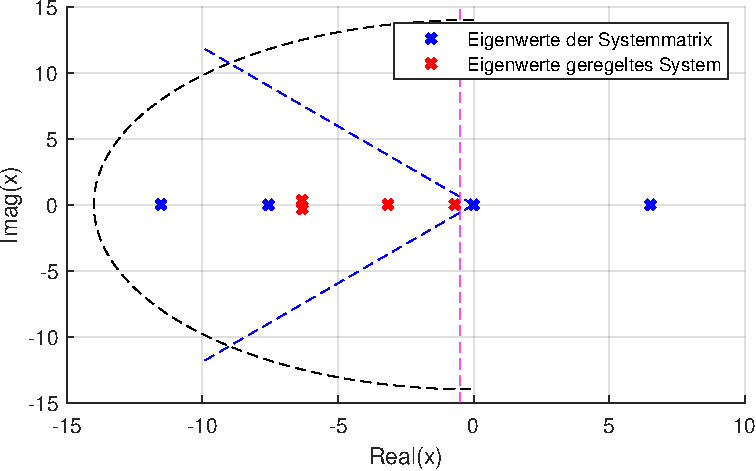
\includegraphics[width=0.8\textwidth]{Bilder/7_zustandsregler/Vergleich_der_Polstellenlagen.pdf}}
   \caption[Polstellenlagen der Systemmatrix und des geschlossenen Regelkreises]{Vergleich der Polstellenlagen der Systemmatrix A und des geschlossenen Regelkreises}
   \label{fig:Bild7.6}
\end{figure}

Der geschlossene Regelkreis weist nur Polstellen mit einem Realteil kleiner Null auf. Folglich ist das System stabil. In \autoref{fig:Bild7.7} sind der Kurvenverlauf des Pendelwinkels $\Theta$, als auch der des Schwungradwinkels $\varphi$ dargestellt. Aus den Kurvenverläufen wird geschlussfolgert, dass die implementierte Reglerstruktur das Pendel in die instabile Ruhelage zurückregelt. Die maximale Eingangsspannung von 20V wird dabei nicht überschritten. Die eingangs gesetzten Regelziele gelten als erfüllt.

\begin{figure}[H]
   \centering
   \fbox{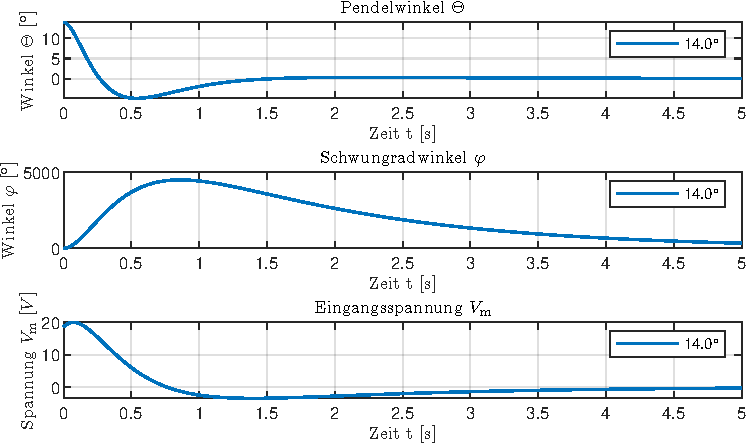
\includegraphics[width=0.95\textwidth]{Bilder/7_zustandsregler/Validierung_des_Reglers.pdf}}
   \caption[Relevante Kurvenverläufe zur Validierung des Reglers]{Relevante Kurvenverläufe zur Validierung des Reglers}
   \label{fig:Bild7.7}
\end{figure}

\subsection{Regleranwendung am nichtlinearen Modell}
\label{sec:Regleranwendung}

Bei der Anwendung des linearen Reglers am nichtlinearen Modell werden die erweiterten LMI-Parameter aus \autoref{eq:Gleichung7.7} angesetzt, d.h. der k-Vektor aus \autoref{eq:Gleichung7.8} gilt. Die relevanten Kurvenverläufe sind in \autoref{fig:Bild7.8} dargestellt. Diese ähneln den Kurvenverläufen aus \autoref{fig:Bild7.7}. Die maximale Eingangsspannung des nichtlinearen Modells ist: $V_{\mathrm{m,Max}} \approx 19.924V$. Die vorgegebenen Constrains sind eingehalten. Der lineare Regler ist in der Lage, das instabile nichtlineare System für Auslenkungen bis 14$^\circ$ zu stabilisieren.

\begin{figure}[H]
   \centering
   \fbox{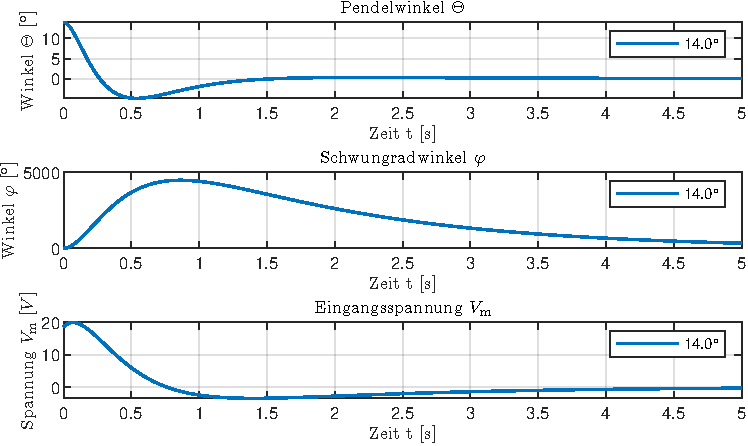
\includegraphics[width=0.95\textwidth]{Bilder/7_zustandsregler/Anwendung_des_Reglers.pdf}}
   \caption[Relevante Kurvenverläufe zur Anwendung des Reglers]{Relevante Kurvenverläufe zur Anwendung des Reglers}
   \label{fig:Bild7.8}
\end{figure}